\documentclass[]{article}

%imports
\usepackage{amsmath}
\usepackage{amsthm}
\usepackage{amssymb}
\usepackage{tikz-cd}
\usepackage{quiver}
\usepackage{array}
\usepackage[all,cmtip]{xy}



\usepackage{hyperref}
\usepackage{cleveref}


\usepackage[style=alphabetic]{biblatex}

%references
\addbibresource{ref.bib}
%\bibliography{ref.bib}

%newtheorems
\theoremstyle{definition}
\newtheorem{definition}{Definition}[section]

\newtheorem{theorem}{Theorem}[section]
\newtheorem{corollary}{Corollary}[section]
\newtheorem{lemma}{Lemma}[section]
\newtheorem{proposition}{Proposition}[section]
\newtheorem{example}{Example}[section]
\newtheorem{question}{Question}

%commands
\newcommand{\mo}{\ensuremath{\text{mod }}}
\newcommand{\Hom}{\ensuremath{\text{Hom}}}
\newcommand{\tu}{\ensuremath{\tau}}
\newcommand{\Fac}{\ensuremath{\text{Fac }}}

\newcommand{\spmat}[1]{%
	\begin{bmatrix}#1\end{bmatrix}%
}




%opening
\title{Computing \tu-rigid modules}
\author{Håvard Utne Terland}

\begin{document}

\maketitle

\begin{abstract}

\end{abstract}

\section{Introduction}
Representation theory of algebras may be understood as understanding the ways a finite set of linear transformations may act together on vector spaces given some constraints. This may formulated using the language of module theory, where systems of linear transformations corresponds to modules over a finite dimensional algebra derived from the class of systems of linear transformations one is studying. To be more precise, this class of systems is given as a quiver, and the constraints are given as an ideal of the path algebra over the quiver.


In these terms, representation theory of algebras then seeks to classify modules over finite dimensional algebras. For special classes of algebras, much progress has been made in this regard. However, the majority of algebras are too complicated for a proper classification of modules to be made.

To give an example, we may consider the quiver below. A representation of this quiver is simply a linear transformation from one finite dimensional vector space to some other finite dimensional vector space.
% https://q.uiver.app/?q=WzAsMixbMCwwLCJcXGJ1bGxldCJdLFsxLDAsIlxcYnVsbGV0Il0sWzAsMV1d
\[\begin{tikzcd}
	1 & 2
	\arrow[from=1-1, to=1-2]
\end{tikzcd}\]

A representation of the above is in other words given by an arbitrary $n \times m$ matrix, over the field one wishes to work over. When dealing with a single linear transformation, classical linear algebra is sufficient, and computing the rank, nullity and corank of the matrix gives you everything we need to understand the transformation (corank for an $n \times m$ matrix is $m$ minus the rank of the matrix). Thus, there is no surprise that there are three indecomposable representations of this quiver, as seen in the figure below. Thus a matrix $M$ corresponds to some number of copies of the representations $M_1,M_2$ and $M_3$. These numbers are exactly the rank, nullity and corank of $M$, respectively.

% https://q.uiver.app/?q=WzAsNixbMCwyLCJcXGJ1bGxldCJdLFsxLDIsIlxcYnVsbGV0Il0sWzAsMSwiXFxidWxsZXQiXSxbMSwxLCJcXGJ1bGxldCJdLFswLDAsIlxcYnVsbGV0Il0sWzEsMCwiXFxidWxsZXQiXSxbMCwxXSxbMiwzXSxbNCw1XV0=
\begin{figure}
	\[\begin{tikzcd}
		M_1: k & k \\
		M_2: k & 0 \\
		M_3: 0 & k
		\arrow[from=3-1, to=3-2,"0"]
		\arrow[from=2-1, to=2-2,"0"]
		\arrow[from=1-1, to=1-2,"1"]
	\end{tikzcd}\]
\caption{The three indecomposable representations of the quiver with one arrow.}

\end{figure}


In this thesis, we focus not on understanding all modules, but instead focus on computing and classifying \tu-rigid modules over as general algebras as our techniques let us. The reasons for studying \tu-rigid modules come from attempt to generalize tilting theory, in particular from the perspective of mutations. Mutations give a combinatorial tool one can employ to understand \tu-tilting modules, similar to the techniques stemming from using Auslander-Reiten quivers to compute module categories. However, we may understand mutation for algebras where we cannot compute the whole AR-quiver. In this sense, \tu-tilting theory offers a new toolbox in the representation theory of algebras.




\section{Preliminaries}
Here we collect some of the necessary prerequisites for reading this thesis, in all majority results and facts not found in \cite{auslander_reiten_smalo_1995} and \cite{assem_skowronski_simson_2006} which we refer two as general references on the representation of finite dimensional algebras.

\subsection{Notation and setting}
We closely follow the notation of \cite{assem_skowronski_simson_2006}. An algebra $A$ will always refer to a finite dimensional algebra over a field $k$, which need not be algebraically closed. All algebras encountered in this thesis will be, unless otherwise stated, on the form $k\Gamma/I$ for some finite quiver $\Gamma$ and admissible ideal $I$. The number $n$ is, unless otherwise stated, reserved for the number of indecomposable projective summands of $A$. By $\mo A$ we denote the category of finite dimensional left $A$-modules (in contrast to \cite{assem_skowronski_simson_2006}, who employ right modules). We implicitly identify $A$-modules to representations of its quiver with relations. We denote by $D$ the duality on modules, and by $\text{Tr}$ the transpose. The Auslander-Reiten translate $D\text{Tr}$ is denoted $\tau$.

A module $M$ is called basic if no two nonzero summands are equal, that is $M \cong A \oplus X \oplus X$ implies $X = 0$. We denote by $|M|$ the number of indecomposable summands of $M$. 

We denote by $hom_A(M,N)$ the dimension of the $k$-vector space $\text{Hom}_A(M,N)$.

\subsection{Approximations}
Approximations are used frequently in the representation theory of algebras. In particular, they are very often used in \tu-tilting theory.

\begin{definition}
	Let $\mathcal{C}$ be a subcategory of $\text{mod} A$.  Let $M$ be an $A$-module, and $X \in \mathcal{C}$. A map $f:X \to M$ is called a \textit{right $\mathcal{C}$-approximation} of $M$ if it is the case that for any $Y \in \mathcal{C}$ and map $g:Y \to M$, there is a map $h:Y \to X$ such that $g = f \circ h$. 
	
	Let $M$ be an $A$-module, and $X \in \mathcal{C}$. A map $f:M \to X$ is called a \textit{left $\mathcal{C}$-approximation} of $M$ if it is the case that for any $Y \in \mathcal{C}$ and map $g:M \to Y$, there is a map $h:X \to Y$ such that $g = h \circ f$. 
	
	A left (right) approximation which is also left (right) minimal as a map is called a minimal left (right) approximation.
	
	If $\mathcal{C} = \text{add } M$ for a module $M$, we shorten $\text{add }M$-approximation to $M$-approximation.
\end{definition}


We say that such a subcategory $\mathcal{C}$ is \textit{contravariantly finite} (resp. \textit{covariantly finite}) if every $A$-module $M$ has a right (resp. left) $\mathcal{C}$-approximation. If $\mathcal{C}$ is both contravariantly and covariantly finite, we call it \textit{functorially finite}.


\begin{example}
	Let $M,N$ be modules in $\text{mod } A$. We may always find a left $M$-approximation of $N$ as follows. $\text{Hom}(N,M)$ is finite dimensional as a $k$-vector space, so pick a basis $F = (f_1,f_2,\dots,f_i)$. Then we have a map $f:N \to \bigoplus_{j= 1}^i M$ given by $f = \begin{bmatrix}
	f_1 \\ \vdots \\ f_i
	\end{bmatrix}$. Given any map $g_r:N \to \bigoplus_{j = 1}^k M_j$ where $M_j$ is a summand of $M$, this map will naturally factor through a map $g:N \to \bigoplus_{j = 1}^k M$, which we may describe as $g = [g_1,g_2,\dots,g_k]$. Since $F$ is a basis for $\text{Hom}(M,N)$, we may write \[g = [a_{1,1}f_1 + \dots + a_{1,i}f_i,\dots,a_{k,1}f_1 + \dots + a_{k,i}f_i]\]
	
	Interpreting $c \in k$ as a map $M \to M$ given by $c \cdot1$ where $1$ is the identity map, we can write $g$ as the composition
	\[g = \begin{bmatrix}
	a_{1,1} & \dots & a_{1,i} \\
	\vdots & \dots & \vdots \\
	a_{k,1} & \dots & a_{k,i}
	\end{bmatrix} \times \begin{bmatrix}
	f_1 \\ \vdots \\ f_i
	\end{bmatrix}
	\]
	
	and thus $g_r$ also factors through as wanted.
\end{example}

We now give an example of a non-trivial, non-minimal left approximation.

\begin{example}
	Let $A$ be the algebra defined by the quiver
	\[
	\begin{tikzcd}
	1 \arrow[r,bend left,"\alpha"] & 2 \arrow[l,bend left,"\beta"]  \\
	\end{tikzcd}
	\]
	
	modulo the relations $r^4 = 0$. Then $\text{Hom}(P(1),P(2))$ has dimension $2$, with maps $f_1(x) = x \beta$ and $f_2(x) =  x\beta\alpha\beta$. Clearly, $f_2 = (\beta\alpha) \circ f_1$. 
	
	Using the construction in the above example, the map $f = \begin{bmatrix} \beta \\ \beta\alpha\beta \end{bmatrix}$ is a left $P(2)$-approximation of $P(1)$. It is not left minimal, however. To see this, consider the endomorphism on $P(2) \oplus P(2)$ given by \[\phi = \begin{bmatrix} 1 & 0 \\ \alpha\beta & 0\end{bmatrix}\]
	
	Then $\phi \circ f = f$, but $\phi$ is not an isomorphism. 
	
	$f_1$ alone, however, is a minimal left approximation.
\end{example}


\section{Tau-tilting theory}
$\tau$-tilting theory was introduced in \cite{tau} as a possible generalization of tilting theory, which has had tremendous impact on the field of representation theory of finite dimensional algebras as a whole. Although first introduced in \cite{tau}, some of the main results of $\tau$-tilting theory stem from (cite smalø). We here recall some important definitions and results from $\tau$-tilting theory. Also, we note that there are other approaches to defining \tu-rigid pairs which are fruitful in other contexts. To make these introductory sections both concise and self-contained, we will not dwell on these alternative approaches to the theory here.  When we need different but equivalent definitions in later sections, references to the literature will be made.

We start by discussing $\tau$-rigid modules, which may be considered the building blocks of $\tau$-tilting theory. 


\begin{definition}
	A module $M$ in $\mo A$ is called $\tau$-rigid if $\Hom(M,\tau M) = 0$.
\end{definition}

First note that the Auslander-Reiten formula gives that \tu-rigid objects must be exceptional objects. Note that $X,Y$ being $\tau$-rigid does not imply $X \oplus Y$ being $\tau$-rigid. In fact, studying how indecomposable $\tau$-rigid modules together form larger $\tau$-rigid modules is part of $\tau$-tilting theory.

\begin{definition}\cite[Definition 0.3]{tau}
	A pair $(M,P)$ where $M$ is basic $\tau$-rigid and $P$ basic projective such that $\Hom_A(P,M) = 0$ is called a  $\tau$-rigid pair.
\end{definition}

Along with this definition follows many conventions. For a  $\tau$-tilting module $T = (M,P)$, $P$ will be denote the projective part of $T$ and $M$ the module part. $T$ is called support \tu-tilting if $|M| + |P| = n$, and almost complete support \tu-tilting if $|M| + |P| = n - 1$. A support \tu-tilting pair with no non-zero projective part may also be denoted a \tu-tilting module. 

For $T_1,T_2$ both \tu-rigid pairs, we consider $T_1$ a summand of $T_2$ is both the module part and the projective part of $T_1$ is a summand of the module part and the projective part of $T_2$ respectively.

\begin{example}
	Since $\tu P = 0$ for any projective module $P$, any projective module is \tu-rigid. As a consequence, $A = \oplus_{i = 1}^n P(i)$ is a \tu-tilting module.	
\end{example}

\begin{example}
	For an hereditary algebra $A$, partial tillting modules coincide with \tu-rigid modules. For $M$ partial tilting, $0 = Ext^1_A(M,M) \cong \Hom_A(M,\tu M)$, where the first equality follows from the definition of tilting-modules and the second equality follows from the Auslander-Reiten formula in the hereditary case.
\end{example}

\subsection{Torsion classes induced by support \tu-modules}
Given a support \tu-tilting pair $(M,P)$, we may consider the modules generated by $M$, $\Fac M$. As in classical tilting theory, this is a torsion class, and we have the following very important result.

\begin{theorem}\cite[Theorem 2.7]{tau}\cite{auslandersmalo81}
	There is a bijection between the set of functorially finite torsion pairs, denoted $\text{f-tors} A$ and support \tu-tilting modules, denoted $\text{s}\tu\text{-tilt} A$, given by sending a support \tu-tilting pair $(M,P)$ to $(\Fac M,M^\perp)$.
\end{theorem}

We order the objects in $\text{f-tors} A$ by inclusion on the torsion classes. Thus $(X_1,Y_1) > (X_2,Y_2)$ if $X_2 \subseteq X_1$. This induces an ordering on $\text{s}\tu A$. We denote by $Q(\text{f-tors} A)$ the Hasse-quiver of the above defined ordering on $\text{f-tors} A$.

\subsection{Mutation}
An essential property of support \tu-tilting modules is that one can \textit{mutate} at each summand. More precisely, one has the following.

\begin{theorem}
	For a almost complete support $\tau$-tilting pair $(M,P)$, there exists exactly two distinct support \tu-tilting pairs $(M_0,P_0)$ and $(M_1,P_1)$.
\end{theorem}

In the above theorem, $(M_0,P_0)$ and $(M_1,P_1)$ are said to be mutations of each other, and we may write $M_1 = \mu_X(M_0)$ where $X$ is the indecomposable summand of $M_0$ that we must replace to get $M_1$; formally, we require $M_0 = X \oplus M$ or $P_0 = X \oplus P$. In this case, we \textit{mutate} at $X$.

\begin{proposition}\cite[Definition-Proposition 2.28]{tau}
	Let $T_1$ and $T_2$ be support \tu-tilting modules which are mutations of each other. Then either $T_1 < T_2$ or $T_ 2 < T_1$. In the first case, we consider $T_2$ a right-mutation of $T_1$ and in the second case we consider $T_2$ a left-mutation of $T_1$. Note that if $T_2$ is a left-mutation of $T_1$, $T_1$ is a right-mutation of $T_2$ and vice versa.
\end{proposition}

\subsection{Mutation quivers}
We use mutation of support \tu-tilting modules to define a quiver storing information about these objects.

\begin{definition}
	The support $\tau$-tilting quiver $Q(\text{s\tu-tilt} A)$ has a vertex for each support \tu-tilting module and an arrow $T_1 \to T_2$ if $T_2$ is a left mutation of $T_1$. 
\end{definition}

In the rest of this subsection, we give examples of mutation quivers and discuss some elementary facts about them.


It turns out that mutation of support \tu-tilting module is compatible with the ordering induced by the set of functorially finite torsion classes.
\begin{proposition}
	$Q(\text{s\tu-tilt} A)$ is isomorphic to $Q(\text{f-tors} A)$.
\end{proposition}

\begin{proof}
	We have an isomorphism between the vertex sets of the two quivers. It is enough to prove that there is an arrow $(T_1,P_1) \to (T_2,P_2)$ if and only if there is an arrow $(\Fac T_1,T_1^\perp) \to (\Fac T_2,T_2^\perp)$.
	
	If there is an arrow $(\Fac T_1,T_1^\perp) \to (\Fac T_2,T_2^\perp)$, we have $\Fac T_2 \subset \Fac T_1$ and no functorially finite torsion class $T \neq T_1,T_2$ such that $\Fac T_2 \subset T \subset \Fac T_1$. By \cite[Theorem 2.33]{tau}, this implies that $(T_2,P_2)$ is a left mutation of $(T_1,P_1)$ and thus there is an arrow $(T_1,P_1) \to (T_2,P_2)$ in $Q(\text{s\tu-tilt} A)$.
	
	By \cite[Theorem 2.33]{tau}, a symmetrical argument proves the other direction.	
\end{proof}

\begin{example}
	As $\Fac A=\text{mod } A$, the support \tu-tilting module $(A,0)$ is the largest element in $Q(\text{f-tors} A)$, and any mutation $\mu_X(A)$ must be a left-mutation.
\end{example}

\begin{example}
	Let $A$ be the path algebra of the disconnected quiver with two points.
	
	\[
	\begin{tikzcd}
	\bullet & \bullet   \\
	\end{tikzcd}
	\]
Then $Q(s\tau\text{-tilt} A)$ may easily be computed to be 

% https://q.uiver.app/?q=WzAsNCxbMSwwLCIoUCgxKVxcb3BsdXMgUCgyKSwwKSJdLFsxLDIsIigwLFAoMSlcXG9wbHVzIFAoMikpIl0sWzIsMSwiKFAoMSksUCgyKSkiXSxbMCwxLCIoUCgyKSxQKDEpKSJdLFswLDNdLFszLDFdLFswLDJdLFsyLDFdXQ==
\[\begin{tikzcd}
& {(P(1)\oplus P(2),0)} \\
{(P(2),P(1))} && {(P(1),P(2))} \\
& {(0,P(1)\oplus P(2))}
\arrow[from=1-2, to=2-1]
\arrow[from=2-1, to=3-2]
\arrow[from=1-2, to=2-3]
\arrow[from=2-3, to=3-2]
\end{tikzcd}\]
\end{example}

We now show how the \tu-tilting theory of a disconnected algebra is determined by its components.

\begin{definition}
	Let $Q_1,Q_2$ be quivers with vertex sets $Q_1^0$, $Q_2^0$ and arrow sets $Q_1^1$, $Q_2^1$. The Cartesian product $Q = Q_1 \mathbin{\Box} Q_2$ is defined as the quiver with vertex set $Q_1^0 \times Q_2^0$ and edges on the form $(x_1,y_1) \to (x_2,y_2)$ such that either $x_1 = x_2$ and $y_1 \to y_2$ is an edge in $Q_2^1$, or $y_1 = y_2$ and $x_1 \to x_2$ is an edge in $Q_1^2$.
	\end{definition}

\begin{lemma}
	Let $\Lambda = A \times B$ be a disconnected algebra. Then $Q(s\tu\text{-tilt} \Lambda) \cong Q(s\tu\text{-tilt} A)\mathbin{\Box}Q(s\tu\text{-tilt} B)$ as quivers.
	\end{lemma}
\begin{proof}
$(M,P) = (M_A \oplus M_B,P_A \oplus P_B)$ is support \tu-tilting over $\Lambda$ if and only if $(M_A,P_A)$ is support \tu-tilting over $A$ and $(M_B,P_B)$ is support \tu-tilting over $B$. This follows from the general fact that the module category of $\Lambda$ is the product of the module category of $A$ and the module category of $B$. More concretely, one can see that computing the Auslander-Reiten translate of $M_A$ in $A$ is essentially exactly the same operation as computing it in $\Lambda$, and this is the only nontrivial observation needed.
	
This allows us to compute $Q(s\tu\text{-tilt} \Lambda)$ as the Cartesian product of $Q(s\tu\text{-tilt} A)$ and $Q(s\tu\text{-tilt} B)$. To see this, let $(X,Y)$ be a point in $Q(s\tu\text{-tilt} A) \mathbin{\Box} Q(s\tu\text{-tilt} B)$ Then $X \oplus Y$ is clearly a point int $Q(s\tu\text{-tilt} \Lambda) $ and vice versa. Thus we have a natural bijection between the graphs, we need to investigate the edges. Let $(X_1,Y) \to (X_2,Y)$ be an edge in $Q(s\tu\text{-tilt} A) \mathbin{\Box} Q(s\tu\text{-tilt} B)$.  Then $(X_1 \oplus Y) \to (X_2 \oplus Y)$ is a valid mutation as only one summand has changed, thus corresponding to an edge in $Q(s\tu\text{-tilt} \Lambda)$, and similarly for edges on the form $(X,Y_1) \to (X,Y_2)$. Since all edges in $Q(s\tu\text{-tilt} A)\mathbin{\Box}Q(s\tu\text{-tilt} B)$ are on one of these forms, and clearly all edges in $Q(s\tu\text{-tilt} \Lambda)$ come from these edges, we have a quiver isomorphism.
 	
\end{proof}

One may also consider the graph-theoretical properties of $Q(\text{s\tu-tilt} A)$ by forgetting the orientation of the edges. From the properties of mutation, it follows at once that the mutation graph is $(n-1)$-regular. It may be finite or infinite. In the finite case the graph is connected\cite[Corollary 3.10]{tau}.

\subsection{g-vectors}
For an indecomposable module $M$, let $P_1 \to P_2 \to M \to 0$ be a minimal projective presentation of $M$, where $P_1 \cong \bigoplus_{i = 1}^n P(i)^{v_i}$ and $P_2 \cong \bigoplus_{i = 1}^n P(i)^{u_i}$. We may consider $(v_1,v_2,\dots,v_n)$ and $(u_1,u_2,\dots,u_n)$ to be vectors describing the building blocks of $P_1$ and $P_2$ respectively. Then we define $g^M$ to be $u - v$. 

\begin{definition}
	For a $\tau$-rigid pair $(M,P)$, its $g$-vector is defined as $g^M - g^P$. 
\end{definition}

Further, we follow \cite{schroll2020tautilting} and define $G$-matrices as follows.

\begin{definition}\cite[Definition 2.4]{schroll2020tautilting}
	For a support \tu-tilting pair $(M,P) = (M_1 \oplus \dots \oplus M_i,P_1 \oplus \dots \oplus P_j)$, we define its G-matrix $G_{(M,P)}$ to be the $n \times n$ matrix $(g^{M_1},g^{M_2},\dots,g^{M_i},-g^{P_1},\dots,-g^{P_j})$, where we consider the $g$-vectors to be column vectors.
	
\end{definition} 

An important property of $g$-vectors is that they uniquely identify $\tau$-rigid pairs\cite[Theorem 5.5]{tau}. This immediately gives a combinatorial proof that the set of indecomposable \tu-rigid objects must be countable (a fact known more generally for the set of exceptional objects up to isomorphism), as there are only countably many integer vectors of dimension $n$. 

Further, $G$-matrices of support \tu-tilting pairs are invertible. This follows immediately from \cite[Theorem 5.1]{tau}.

Another often-used fact is the following result.

\begin{theorem}\cite{auslander1985modules}[Theorem 1.4(a)]
	Let $M,N$ be modules. We have \[\langle g^M,[N]\rangle = hom_A(M,N) - hom_A(N,\tau M))\]
\end{theorem}


\subsection{Duality}
There is a duality between the \tu-tilting of $A$ and the \tu-tilting of $A^\text{op}$.

\section{Jasso reduction}
Using techniques from classical tilting theory, Gustavo Jasso\cite{jassoreduction} introduced reduction techniques, now often called Jasso reduction, for partial support \tu-tilting modules, and showed that one can relate the \tu-tilting theory of $A$ to the \tu-tilting theory of these reduced algebras.

This theory is now fundamental to \tu-tilting theory. Here we recall some important aspects of Jasso reduction, and refer to the original paper for a more detailed account.

Let $M$ be a basic \tu-rigid module with $k$ summands. The \textit{Jasso perpendicular} subcategory $J(M)$ is defined as \[J(M) = M^\perp \cap \, ^{\perp}\tau M\]

Jasso has shown that $J(M)$ is equivalent to a module category $\text{mod} \Lambda$ where $\Lambda$. We may obtain $\Lambda$ the following way. Let $B = M \oplus N$ be the Bongartz completion of $M$. Then let $\Lambda = \text{End}_A(B,B)/e_M$, where $e_M$ is the idempotent associated to the projective $\text{End}_A(B,B)$-module $\text{Hom}_A(B,M)$.


\begin{theorem}\cite[Theorem 3.15]{jassoreduction}
	Let $M$ be a basic \tu-rigid module. There is a bijection between the support \tu-tilting modules of $A$ having $M$ as a summand and the support \tu-tilting modules of the algebra with module category $C(M)$. Further, this bijection is order-preserving and respects mutation.
\end{theorem}

We may extend Jasso reduction to partial support \tu-tilting objects, not only \tu-rigid modules by the fact that that a partial support \tu-tilting object $(M,P)$ over $A$ is a \tu-rigid $A/e$-module where $e$ is the idempotent associated to $P$t\cite{tau}.

The above theorem shows that we can understand the \tu-tilting theory of module categories on the form $J(T)$ via the \tu-tilting theory of the whole module category. 

\begin{corollary}
	Let $A$ be a \tu-tilting finite algebra, and $T$ a partial support \tu-tilting module. Let $B$ be the algebra with module category $J(T)$. Then $B$ is \tu-tilting finite.
\end{corollary}

\begin{proof}
	Since we may embed the mutation quiver $Q = Q(s\tu\text{-tilt} B)$ in the finite quiver $Q(s\tu\text{-tilt} A)$, $Q$ itself must be finite.
\end{proof}

\subsection{Brick labeling through Jasso reduction}
If there is an edge $e$ between two support \tu-tilting modules $T_1 = (M_1,P_1)$ and $T_2 = (M_2,P_2)$ in $Q(s\tu\text{-tilt} A)$, there is an almost complete support \tu-tilting object $T = (M,P)$ which is a summand of both $T_1$ and $T_2$. Then $J(T)$ is the module category of a local algebra. The unique simple module $S$ in this category is then a brick in $J(T)$. Since we embed $J(T)$ fully in $\text{mod} A$, $\text{Hom}_{J(T)}(S,S) = \text{Hom}_A(S,S)$, so $S$ is a brick also in $A$. We associate to the edge $e$ this module $S$. This association is called the \textit{brick-labeling} of edges of the mutation quiver.

\section{The wall and chamber structure of finite dimensional algebras}
We here introduce the wall and chamber structure of a finite dimensional algebra $A$, and recall how it may be used to study the \tu-tilting theory of $A$.

\subsection{Stability conditions}

\begin{definition}
	For $v \in \mathbb{R}^n$, a module $M \in \text{mod} A$ is called \textit{$v$-stable} if $\langle v,[M]\rangle = 0$ and $\langle v,[N]\rangle < 0$ for all proper submodules $N$. $M$ is called \textit{$v$-semistable} if $\langle v, [M]\rangle = 0$ and $\langle v, [N]\rangle \leq 0$ for every submodule $N$.
\end{definition}

We denote by $\mathcal{D}(M)$ the set of vectors $v \in \mathbb{R}^n$ such that $M$ is $v$-semistable. We call $\mathcal{D}(M)$ the stability space of $M$.


Stability spaces need not be linear spaces. However, they are always closed under positive scaling and induce linear spaces as their span. The \textit{walls} of the wall and chamber structure of A are defined as the stability spaces which induce linear spaces of codimension 1. We now describe the chambers.

Let $X^c$ denote the compliment of a set $X$ in a topological space, and $\overline{X}$ its closure. We let $\mathcal{R} = (\overline{(\cup_{M \in \text{mod} A} \mathcal{D}(M))})^c$. A \textit{chamber} in the wall and chamber structure of $A$ is defined to be a connected component of $\mathcal{R}$.

We now show that all walls are given by stability spaces of indecomposable modules, before demonstrating some examples.

\begin{proposition}
	$\mathcal{D}(M)$ be a wall. Then there is an indecomposable module $X$ such that $\mathcal{D}(M) = \mathcal{D}(X)$.
\end{proposition}

\begin{proof}
	If $M$ is indecomposable, we let $X = M$. If not, let $M = X\oplus N$, where $N,X \neq 0$. Let $v \in \mathcal{D}(M)$. Then $\langle v,[X]\rangle \leq 0$ and $\langle v,[M]\rangle \leq 0$. Since $\langle v,[M]\rangle = \langle v,[X]\rangle + \langle v,[N]\rangle = 0$, we see that $v \in \mathcal{D}(X)$. Since $[X] \neq 0$, $\mathcal{D}(X)$ must have co-dimension 1. This completes the proof.
\end{proof}

\begin{example}
	Let $A = A_2$. We compute its wall and chamber structure. We have three indecomposable $A$-modules, $S(1),S(2)$ and $P(1)$. Clearly $\mathcal{D}(S(1)) = \{(0,y): y \in \mathbb{R}\}$ and $\mathcal{D}(S(2)) = \{(x,0): x \in \mathbb{R}\}$. We now compute $\mathcal{D}(P(1))$. Let $(x,y) = v \in \mathcal{D}(P(1))$. We then require $\langle v,(1,1)\rangle = 0$ and $\langle v,(0,1)\rangle \leq 0$. The second condition implies that $y \leq 0$. The first condition implies that $x = -y$, and these two conditions are sufficient for $v$ to be in the stability space of $P(1)$. Thus the stability space of $P(2)$ is the ray $\{\alpha(1,-1) :  \alpha \in \mathbb{R}, \alpha \geq 0\}$. 
\end{example}


\subsection{Cones, walls and chambers induced by \tu-tilting pairs}
We now aim to recover information about the \tu-tilting theory of an algebra from its wall and chamber structure.

An important ingredient in this section is the following formula.
\begin{proposition}
	Let $(M,P)$ be a \tu-rigid pair. Then
 \[\langle g^{(M,P)},[N]\rangle = hom_A(M,N) - hom_A(N,\tau M) - hom_A(P,N)\]
\end{proposition}

\begin{proof}
	The proposition follows from applying \cite{auslander1985modules}[Theorem 1.4(a)] twice.
\end{proof}

Note that the above formula implies that a diension vector $[X]$ with $X$ in $J(M,P) = J(M_1\oplus\dots\oplus M_i,P_1\oplus\dots\oplus P_j)$ will be orthogonal to $g^{(M,P)}$. Also, by additivity, $[X]$ will be orthogonal to any linear combination of the vectors $\{g^{M_1},\dots,g^{M_i},-g^{P_1},\dots,-g^{P_j}\}$. We now aim to prove a partial converse to this statement.
\begin{definition}
	Let $T = (M,P)$ be a \tu-rigid pair. We define the \textit{cone} spanned by $T$, as \[C(T) = \{\sum_{i = 1}^{j} \alpha_ig^{M_i} - \sum_{i = 1}^{k}\beta_ig^{P_i} : \alpha_i,\beta_i \geq 0 \text{ for all } i\}\]
	
	The interior $C^\circ(T) \subset C(T)$ is defined by requiring all coefficients $\alpha_i,\beta_i$ to be strictly positive.
\end{definition} 

Given a vector $\alpha = (\alpha_1,\alpha_2,\dots,\alpha_n)$ with $\alpha_i \geq 0$ for all $i$, we let $\alpha(M,P)$ denote the vector $G^{(M,P)} \times \alpha$.

\begin{proposition}\cite{Br_stle_2019}[Proposition 3.13]
	For $\alpha(M,P) \in C^\circ(M,P)$, a module $N$ is $\alpha(M,P)$-semistable if and only if $N \in J(M,P)$.
\end{proposition}

Note that the simple objects in $J(M,P)$ are, by the proposition above, exactly the $\alpha(M,P)$-stable modules.

\begin{question}
	Can we find the $\alpha(M,P)$-stable modules? Doing this would allow us to say something about the correspondence between dimensions vectors of $J(M,P)$-objects as embedded in $\text{mod} A$ versus their embedding in $\text{mod} C = J(M,P)$ for the appropriate algebra $C$.
\end{question}



The cones $C(T)$ for support \tu-tilting modules and almost complete support \tu-tilting modules play an important role in the wall and chamber structure of an algebra.

\begin{proposition}\cite[Proposition 3.15, Corollary 3.16, Corollary 3.21]{Br_stle_2019}\label{tau-wall-chamber-result}
	\begin{enumerate}
		\item For a support \tu-tilting object $T_1 = (M,P)$, $C^\circ(T_1)$ defines a chamber in the wall and chamber structure of $A$.
		\item For an almost complete support \tu-tilting object $T_2 = (M,P)$, $C(T_2)$ is included in a wall $\mathcal{D}(N)$ in the wall and chamber structure of $A$. The module $N$ may be computed given the two support \tu-tilting modules containing $(M,P)$.
		\item For \tu-tilting finite algebras, all chambers are on the form $C^\circ(T)$ for a support \tu-tilting object $T$.
		
	\end{enumerate}
\end{proposition}


\begin{example}
	Consider the Kronecker algebra $K_2$. Let $M$ be an indecomposable module with dimension vector $(1,1)$. Then $\mathcal{D}(M) = \{(-1,1)\}$. However, there is no \tu-rigid module with $g$-vector $(-1,1)$, as $\text{Hom}_A(P(1),P(2)) = 0$.
\end{example}


Using the third point of \cref{tau-wall-chamber-result}, we may conclude that an algebra with infinitely many walls in its wall and chamber structure will be \tu-tilting infinite. It is well known that algebras whose quivers have a double arrow are representation infinite. Here we show that they are \tu-tilting infinite as well.
\begin{proposition}
	Any algebra $A = k\Gamma/I$ where $\Gamma$ has a double arrow is \tu-tilting infinite.
\end{proposition}

\begin{proof}
	We note that the proof is very much inspired by the proof of \cite[Theorem 4.14]{Br_stle_2019}. Label the vertices of $\Gamma$ such that the double arrows are from $1 \to 2$. Then any module over $K_2$ may be canonically embedded as a module of $A$, and in particular we have for any $n \geq 2$ a module $M_n$ with dimension vector $x = (n,n+1,0,\dots,0)$, such that its proper submodules have dimension vectors $(n-k,n+1-k,0,\dots,0)$ for $1 \leq k \leq n$. We investigate $D(M_n)$.
	
	Let $v = (v_1,v_2,\dots,v_n) \in D(M_n)$. We have $\langle v,x \rangle = 0$ and $\langle v,x - (k,k,0,0,\dots,0)\rangle \leq 0$ for all integers $1 \leq k \leq n$. Thus for $i > 2$, $v_i$ may be chosen freely. Also, letting $k = n$ in the second condition, we see that $v_2 \leq 0$. The first condition implies $v_1 = \frac{-(n+1)}{n}v_2$.
	
	Assume now that $y = (y_1,y_2,\dots,y_n)$ such that the two above properties hold, namely $y_2 \leq 0$ and $y_1 = \frac{-(n+1)}{n}y_2$. We then clearly have $\langle y,[M]\rangle = 0$. We now check that for all $N \subseteq M$, we have $\langle y,[N]\rangle \leq 0$. 
	
	\begin{align}
	&\langle (\frac{-(n+1)}{n}y_2,y_2), (n-k,n+1-k)\rangle \\
	=&\langle (\frac{-(n+1)}{n}y_2,y_2), (j,j+1)\rangle \\
	=& y_2((-nj-j)/n + (j+1)) \\
	=& y_2((-nj - j + nj + n)/n) \\
	=& y_2((n-j)/n)) \\
	\leq& 0\text{, since } j \leq n
	\end{align}
	
	Thus $y$ is in $D(M_n)$. Since we may chose $y_i$ for $i > 2$ freely, and any non-positive $y_2$, $D(M_n)$ generates a linear space of codimension $1$, and is thus a wall in the wall and chamber structure of $A$.
	
	Further, letting $m,n \geq 1$, it is easy to see that $D(M_n) = D(M_m)$ implies $m = n$. Thus we have identified an infinite number of walls in the wall and chamber structure of $A$, meaning that $A$ is \tu-tilting infinite.
	
\end{proof}


\subsection{Consequences for the structure of $Q(s\tu\text{-tilt})$}


This following result shows that cones of $\tau$-rigid objects intersect in a very controlled fashion.

\begin{proposition}\cite[Corollary 6.7, b)]{dij17}
	Let $T_1,T_2$ be support \tu-tilting objects. Then $C(T_1) \cap C(T_2) = C(X)$ with $X$ being the maximal \tu-rigid pair such that $X$ is a summand of $T_1$ and of $T_2$.
\end{proposition}

\begin{proof}
\end{proof}


This result gives a tool for classifying all support \tu-tilting objects. We collect this technique as a theorem.

\begin{theorem}\cite{dij17}
	Let $A$ be an algebra.
	
	\begin{itemize}
		\item If $A$ is \tu-tilting finite, its mutation graph is connected, thus the set of support \tu-tilting modules over $A$ are exactly the ones in this component.
		\item If it is \tu-tilting infinite the mutation graph may be disconnected. Let $X$ be a set of support \tu-tilting modules such that $\cup_{T \in X} C(T)$ is dense in $\mathbb{R}^n$. Then $X$ contains all support \tu-tilting modules over $A$.
		
	\end{itemize}
\end{theorem}

\begin{proof}
	The \tu-tilting finite case is well-known. We note that the second point also holds in this case, but is not needed as connectivity of the mutation graph is sufficient to to compute all support \tu-tilting modules.
	
	Let $T = (M,P)$ be a support \tu-tilting object. Consider a point $x \in C(T)$ in the interior of $C(T)$. Since $\cup_{T \in X} C(T)$ is dense in $\mathbb{R}^n$, there is a $T_2$ in $X$ such that $C(T_2) \cap C(T)$ contains $x$. But $C(T_2)\cap C(T) = C(Y)$ for some partial suport \tu-tilting object $Y$. Since $T \neq T_2$, there is a summand $Z$ in $T = (M,P)$ not in $Y$. Writing $x$ as an element of $C(T)$, we get
	
	\[x = \sum_{i = 1}^{j} \alpha_ig^{M_i} - \sum_{i = 1}^{k}\beta_ig^{P_i}\]

	The above expression also gives a way of writing $x$ as an element of  $C(T)$, where in particular the $g^{Z}$ coordinates are $0$. Thus $x$ lies on the border of $C(T)$, giving us a contradiction.
	
\end{proof}

It is interesting to note that the converse to the above theorem holds for tame algebras, though not in general\cite{keller2020tame}.

in \cite{dij17}, the authors use the above demonstrated criteria to classify the support \tu-tilting objects of two specific symmetric algebras. 

We may also use the wall and chamber structure to detect the non-existence of maximal green sequences. A maximal green sequence in $Q(s\tu\text{-tilt})$ is a path from $(A,0)$ to $(0,A)$. If there is no such path, the mutation quiver has at least two connected components.

By \cref{tau-wall-chamber-result}, a path in the mutation quiver gives rise to a sequence of chambers where neighboring chambers share a wall. In \cite{Br_stle_2019}, the authors define $\mathcal{D}$-generic paths as certain paths $\gamma:[0,1] \to \mathbb{R}^n$ starting and ending in chambers, essentially passing only one wall at a time and doing so transversely. They then demonstrate that a maximal green sequence gives rise to such a $\mathcal{D}$-generic sequence from the chamber induced by $(A,0)$ to the chamber induced by $(0,A)$.


\subsection{Main results}
We now exploit the techniques discussed so far to determine properties of mutation quivers $Q(s\tau\text{-tilt} A)$ for various algebras $A$.


\subsection{Inheriting mutation from Kronecker algebras}
The idea of the following theorem is to use the \tu-tilting theory of the Kronecker algebra with two arrows, $K_2$, to explicitly compute mutations in a more complicated algebra.

\begin{theorem}\label{k2-reduction}
	Let $A$ be an algebra on the form $kQ/r^2$ where $Q$ is the quiver	
	\[\begin{tikzcd}
	1 
	\arrow[r,bend left,shift right = 0.5ex, "\beta"]
	\arrow[r,bend left, shift left = 2ex, "\alpha"]
	& 2 \arrow[l,bend left,shift right = 0.5ex,"\gamma"]
	\arrow[l,bend left,shift left = 2ex, "\delta"]  \\
		\end{tikzcd}
	\]
	
	Then $Q(s\tau\text{-tilt } A)$ has exactly two components.
		
\end{theorem}



\begin{proof}
	A module $M$ over $A$ where either the maps induced by $\gamma$ and $\delta$, or $\alpha$ and $\beta$ are zero may naturally be considered a $K_2$-module.
	
	Then it is not difficult to see that the $g$-vector of such an $M$ as a $K_2$-module is the same as the $g$-vector of $M$ as an $A$-module, up to switching coordinates (if we demand that arrows go from vertex $1$ to $2$ in $K_2$, we need to do this swap for the case where $M$ is an $A$-module where $\alpha,\beta$ are zero).
	
	Consider the mutation of $P(1) \oplus P(2)$ at $P(1)$.
	
	\[P(1) \xrightarrow{\begin{bmatrix} \gamma \\ \delta\end{bmatrix}} P(2) \oplus P(2)\]
	
	Is a minimal right $P(2)$-approximation of $P(1)$, and its cokernel $X$ is naturally a $K_2$ module, as $\alpha X = 0$, and $\beta X= 0$. It is also $\tau$-rigid as a $K_2$ module. We thus have a \tu-tilting pair $T = (P(2),X)$ over $A$, which may naturally be considered a \tu-tilting pair over $K_2$. 
	
	This means that all iterated left mutations from $T$ are controlled by mutation in $K_2$. 
	
	A symmetrical argument shows that mutating $P(1) \oplus P(2)$ at $P(2)$ gives a \tu-tilting module whose iterated left-mutations are again dictated by mutation on $K_2$.
	
	Thus we may compute the $g$-vectors of these \tu-tilting modules, as shown in the figure.
	
	
		\begin{figure}
			\begin{center}
			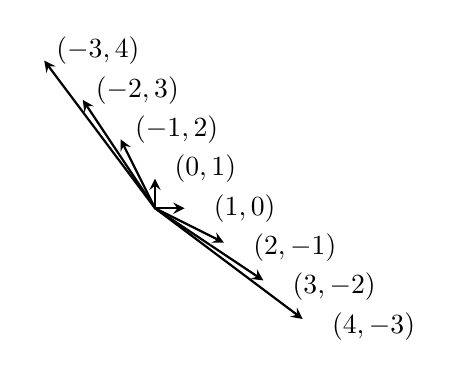
\begin{tikzpicture}[>=stealth,scale=0.5,line cap=round,
		bullet/.style={circle,inner sep=1.5pt,fill}]
		%\draw[->] (-5,0) -- (5,0) node[right]{$x$};
		%\draw[->] (0,-5) -- (0,5) node[above]{$y$};
		%\draw foreach \X in {3,6}
		%{(\X,0.1) -- ++ (0,-0.2) node[below]{$\X$}};
		%\draw foreach \Y in {2,4}
		%{(0.1,\Y) -- ++ (-0.2,0) node[left]{$\Y$}};
		\foreach \X [count=\Y] in {(1,0),(0,1),(-1,2),(-2,3),(-3,4),(2,-1),(3,-2),(4,-3)} 
		{\path  \X node(n\Y)[label=right:{$\X$}]{};
			\draw[thick,->]  (0,0) -- (n\Y);}
		\end{tikzpicture}
			\end{center}
		\caption{The $g$-vectors given by indecomposable summands of support \tu-tilting objects at most three left mutations from $(P(1) \oplus P(2),0)$ for the algebra $A$}
		\end{figure}
	
	The closure of the cones coming from the support \tu-tilting objects which are left mutations of $P(1) \oplus P(2)$ clearly hit any point $(x,y) \in \mathbb{R}^2$ where $y + x \geq 0$. 
	
	Since $A$ is symmetrical, we have $g^{((M,P)^\dagger)^\text{op}} = -g^{(M,P)}$. Thus the closure of the cones coming from right-mutations at $(0,P(1) \oplus P(2))$ hits any point where $y + x \leq 0$. 
	
	Thus we see that all points $(x,y) \in \mathbb{R}^2$ lies in the closure of the cones coming from support \tu-tilting objects in these two components. This concludes the proof.
	
	
\end{proof}

We may generalize the theorem above slightly.
\begin{corollary}
	Let $A_{i,j}$ be the algebra on the form $kQ/r^2$ where $Q$ is on the form
	\[\begin{tikzcd}
	1
	\arrow[r, shift right = -3.5ex, draw=none, "\raisebox{+2.5ex}{\vdots}" description]
	\arrow[r,bend left,shift right = 0.5ex, "\alpha_i"]
	\arrow[r,bend left, shift left = 4ex, "\alpha_1"]
	& 2 \arrow[l, shift left = 5.0ex, draw=none, "\raisebox{+2.5ex}{\vdots}" description]
	\arrow[l,bend left,shift right = 0.5ex,"\beta_j"]
	\arrow[l,bend left,shift left = 4.0ex, "\beta_1"]  \\
	\end{tikzcd}
	\]
	
	Then $Q(s\tu\text{-tilt} A_{i,j})$ has exactly two connected components for all $i,j \geq 2$.
	
\end{corollary}

\begin{proof}
Entirely equivalent to the case where $i = 2 = j$, we will still have that left mutations of $P(1) \oplus P(2)$  behave as if they were left mutations appearing in the Kronecker algebra case.

	\begin{figure}
	\begin{center}
		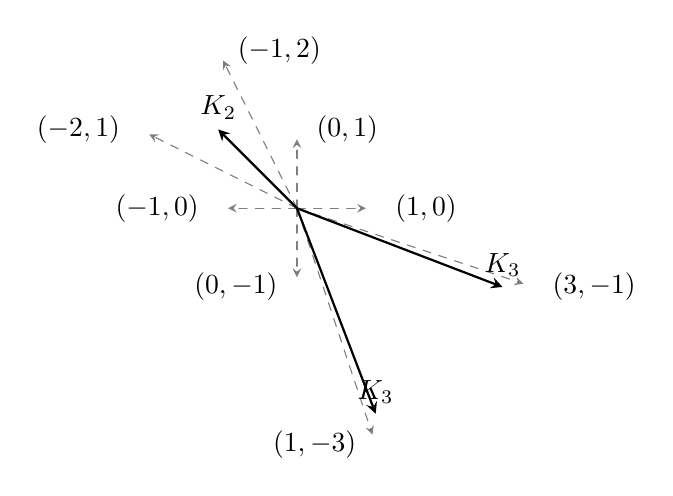
\begin{tikzpicture}[>=stealth,scale=1,line cap=round,
		bullet/.style={circle,inner sep=1.5pt,fill}]
		%\draw[->] (-5,0) -- (5,0) node[right]{$x$};
		\draw[thick,->] (0,0) -- (2.61,-1) node[above]{$K_3$};
		\draw[thick,->] (0,0) -- (1,-2.61) node[above]{$K_3$};
		\draw[thick,->] (0,0) -- (-1,1) node[above]{$K_2$};
		%\draw foreach \X in {3,6}
		%{(\X,0.1) -- ++ (0,-0.2) node[below]{$\X$}};
		%\draw foreach \Y in {2,4}
		%{(0.1,\Y) -- ++ (-0.2,0) node[left]{$\Y$}};
		\foreach \X [count=\Y] in {(1,0),(0,1),(-1,2),(3,-1)} 
		{\path  \X node(n\Y)[label=right:{$\X$}]{};
			\draw[dashed,->,opacity = 0.5]  (0,0) -- (n\Y);}
		
			\foreach \X [count=\Y] in {(-1,0),(0,-1),(-2,1),(1,-3)} 
		{\path  \X node(n\Y)[label=left:{$\X$}]{};
			\draw[dashed,->,opacity = 0.5]  (0,0) -- (n\Y);}
		\end{tikzpicture}
	\end{center}
	\caption{The $g$-vectors given by indecomposable summands of support \tu-tilting objects at most two left mutations from $(P(1) \oplus P(2),0)$ or two right mutations from $(0,P(1)\oplus P(2))$ for the algebra $A_{3,2}$. The area between the vectors labeled $K_3$ is densely filled with walls.}
\end{figure}

The $g$-vectors of right mutations from $(0,P(1)\oplus P(2))$ may be computed indirectly by left mutations of $(P(1)^*\oplus P(2)^*,0)$ on $A^\text{op}$. 

Note that a wall $v$ in $K_i$  gives a wall $v$ in $A_{i,j}$. Also, a wall $w_1 = (x,y)$ in $K_j$ gives a wall $w_2 = (y,x)$ in $A_{i,j}$ because we need to swap the arrows in $K_j$ to view it as a quotient of $A_{i,j}$.

The closure cones of the identified support \tu-tilting objects now span $\mathbb{R}^2 - C(W)$, were $C(W)$ is the closure of all walls. Thus by (......), these are all support \tu-tilting objects.


\end{proof}

The following corollary gives an example of an algebra with more than two components in its \tu-tilting mutation quiver.

\begin{corollary}
	Let $A$ be the algebra on the form $kQ/r^2$ with the quiver.
	
	% https://q.uiver.app/?q=WzAsNCxbMCwwLCJcXGJ1bGxldCJdLFswLDEsIlxcYnVsbGV0Il0sWzIsMCwiXFxidWxsZXQiXSxbMiwxLCJcXGJ1bGxldCJdLFswLDEsIiIsMix7ImN1cnZlIjoxfV0sWzAsMSwiIiwwLHsiY3VydmUiOjJ9XSxbMSwwLCIiLDEseyJjdXJ2ZSI6MX1dLFsxLDAsIiIsMSx7ImN1cnZlIjoyfV0sWzIsMywiIiwxLHsiY3VydmUiOjF9XSxbMiwzLCIiLDEseyJjdXJ2ZSI6Mn1dLFszLDIsIiIsMSx7ImN1cnZlIjoxfV0sWzMsMiwiIiwxLHsiY3VydmUiOjJ9XSxbMCwyXV0=
	\[\begin{tikzcd}
	1 && 3 \\
	2 && 4
	\arrow[curve={height= 6pt}, from=1-1, to=2-1]
	\arrow[curve={height=12pt}, from=1-1, to=2-1]
	\arrow[curve={height=6pt}, from=2-1, to=1-1]
	\arrow[curve={height=12pt}, from=2-1, to=1-1]
	\arrow[curve={height=6pt}, from=1-3, to=2-3]
	\arrow[curve={height=12pt}, from=1-3, to=2-3]
	\arrow[curve={height=6pt}, from=2-3, to=1-3]
	\arrow[curve={height=12pt}, from=2-3, to=1-3]
	%\arrow[from=1-1, to=1-3]
	\end{tikzcd}\]
	
	Then $Q(s\tau\text{-tilt} A)$ has exactly $4$ connected components.
\end{corollary}

\begin{proof}
	Let $A_1 = P(1) \oplus P(2)$, $A_2 = P(3) \oplus P(4)$. Let $Q = Q(s\tu\text{-tilt} A)$.
	
	Then $Q(s\tu\text{-tilt} A)$ is, as a directed graph, the cartesian product of $Q(s\tu\text{-tilt} \text{End}(A_1))$ and $Q(s\tu\text{-tilt} \text{End}(A_2))$. Each of these have two connected components, so its product has four.
	
	More concretely, it is not hard to see that every support \tu-tilting object lies in the same components as either $(A_1\oplus A_2,0)$, $(A_1,A_2)$, $(A_2,A_1)$ or $(0,A_1 \oplus A_2)$ and that none of these four objects lie in the same component.
\end{proof}

We now discuss one consequence of the above result. It it natural to seek an algorithm which enumerates all support \tu-tilting objects. For algebras $A$ where every support \tu-tilting object may be found in the same component as $(A,0)$ or $(0,A)$, this can be done by recursively left-mutating and right-mutating at $(A,0)$ and at $(0,A)$. The above corollary demonstrates that this algorithm does not in general enumerate all support \tu-tilting objects.

There are also connected algebras with more than two components in its \tu-tilting mutation quiver.

\begin{corollary}
	Let $A$ be the algbera on the form $kQ/r^2$ with $Q$ as the quiver below.
	
	% https://q.uiver.app/?q=WzAsNCxbMCwwLCJcXGJ1bGxldCJdLFswLDEsIlxcYnVsbGV0Il0sWzIsMCwiXFxidWxsZXQiXSxbMiwxLCJcXGJ1bGxldCJdLFswLDEsIiIsMix7ImN1cnZlIjoxfV0sWzAsMSwiIiwwLHsiY3VydmUiOjJ9XSxbMSwwLCIiLDEseyJjdXJ2ZSI6MX1dLFsxLDAsIiIsMSx7ImN1cnZlIjoyfV0sWzIsMywiIiwxLHsiY3VydmUiOjF9XSxbMiwzLCIiLDEseyJjdXJ2ZSI6Mn1dLFszLDIsIiIsMSx7ImN1cnZlIjoxfV0sWzMsMiwiIiwxLHsiY3VydmUiOjJ9XSxbMCwyXV0=
	\[\begin{tikzcd}
	1 && 3 \\
	2 && 4
	\arrow[curve={height= 6pt}, from=1-1, to=2-1]
	\arrow[curve={height=12pt}, from=1-1, to=2-1]
	\arrow[curve={height=6pt}, from=2-1, to=1-1]
	\arrow[curve={height=12pt}, from=2-1, to=1-1]
	\arrow[curve={height=6pt}, from=1-3, to=2-3]
	\arrow[curve={height=12pt}, from=1-3, to=2-3]
	\arrow[curve={height=6pt}, from=2-3, to=1-3]
	\arrow[curve={height=12pt}, from=2-3, to=1-3]
	\arrow[from=1-1, to=1-3]
	\end{tikzcd}\]
	
	Then $Q(s\tau\text{-tilt} A)$ has at least $3$ connected components.
\end{corollary}

\begin{proof}
	We use GAP to verify that there is a \tu-tilting object $T = X \oplus P(2) \oplus P(3) \oplus P(4)$ where $X$ has dimension vector $(3,2,0,0)$.
	Then $T = (X_1 \oplus P(2), P(3) \oplus P(4))$ is a support \tu-tilting object. We intend now to show that it may not lie within a finite number of right or left mutations from $(A,0)$ and from $(0,A)$. This means in turn that $T$ must lie in a third component of $Q(s\tu\text{-tilt} A)$, as wanted.
	
	From \cite{Br_stle_2019}[Lemma 4.13], we see that a wall in the wall and chamber structure of the algebra presented in corollary 5.1, call this algebra $B$, gives a wall in the wall and chamber structure of $A$.
	
	
	$g^T$ lies in the cone of a support \tu-tilting module in the same component as $T_B = (P(1)\oplus P(2),P(3) \oplus P(4)$ in $B$. By inspection (Use the result of Asai instead?), we see that any $\mathcal{D}$-generic path from $g^{T_B}$ to $g^{(B,0)}$ or $g^{(0,B)}$ in the wall and chamber structure of $B$ must cross infinitely many walls. This must be inherited in $A$. So any $\mathcal{D}$-generic path from $g^T$ to $(g^{(A,0)}$ or $g^{(0,A}$ must pass an infinite amount of walls. And thus $T$ cannot lie in the same component as $g^{(A,0)}$ or $g^{(0,A)}$, by the converse of \cite{Br_stle_2019}[Lemma 4.2].
	
	
\end{proof}

\subsection{Further reductions}
We will here generalize the main theorem of the above subsection, \cref{k2-reduction}. Note that if we wish to study the algebra $A = kQ/r^3$ with $Q$ being the quiver

\[\begin{tikzcd}
	1 
	\arrow[r,bend left,shift right = 0.5ex, "\beta"]
	\arrow[r,bend left, shift left = 2ex, "\alpha"]
	& 2 \arrow[l,bend left,shift right = 0.5ex,"\gamma"]
	\arrow[l,bend left,shift left = 2ex, "\delta"]  \\
\end{tikzcd}
\]

we can no longer use the same proof as for\cref{k2-reduction} to compute its mutation quiver. In the theorem below, we will demonstrate that we may still use data from $K_2$ to compute $Q(s\tu\text{-tilt} A)$, but the reduction becomes visible not so much directly in the module category but rather in the bounded homotopy category $K^b(\text{add } A)$.

\begin{theorem}
	Let $A = kQ/I$ be an algebra where $Q$ is as follows, and $I$ is an admissible ideal with $r^3 \subseteq I$. Where $r$ is the radical of $kQ$. Then $Q(s\tu\text{-tilt} A)$ has exactly two components.
\[\begin{tikzcd}
	1 
	\arrow[r,bend left,shift right = 0.5ex, "\beta"]
	\arrow[r,bend left, shift left = 2ex, "\alpha"]
	& 2 \arrow[l,bend left,shift right = 0.5ex,"\gamma"]
	\arrow[l,bend left,shift left = 2ex, "\delta"]  \\
\end{tikzcd}
\]
\end{theorem}

Before proving this theorem, we need some lemmas of independent interest.

\begin{lemma}\label{2term-reduction}
	Let $A$ be an algebra over some quiver with some ordering of its vertices, such that $\text{Hom}(P(2),P(1))$ is $2$-dimensional.
	
	Then there is for any non-negative integer $n$ a rigid complex in $K^b(\text{add} A)$, $\mathbb{P}_A(n)$ on the form \[nP(2) \to (n+1)P(2)\]

\end{lemma}

\begin{proof}
	The case where $n = 0$ is trivial, so assume that $n \geq 1$. Let first $K$ be the Kronecker algebra with two arrows. Let now $\mathbb{P}_K $ be the complex \[nP_K(2) \xrightarrow{f} (n+1)P_K(1)\] be a rigid 2-term complex over. Note that $f$ may be viewed as an $n\times(n+1)$ matrix over $\text{Hom}_K(P(2),P(1)$ which is $2$-dimensional. Pick an isomorphism $\phi$ between $\text{Hom}_K(P(2),P(1))$ and $\text{Hom}_A(P(2),P(1))$. Then we may let $\phi$ act entry-wise on $f$. Call this induced map $\phi(f)$. We claim now that the complex $\mathbb{P}_A$ given by  \[nP_A(2) \xrightarrow{\phi(f)} (n+1)P_A(1)\] is rigid.
	
	To check rigidity of $\mathbb{P}_A$, we must show that $\text{Hom}_{K^b(\text{add} A)}(\mathbb{P}_A,\mathbb{P}_A[1]) = 0$, meaning that all maps from $\mathbb{P}_A$ to $\mathbb{P}_A$ shifted should be null-homotopic. Let now $g:nP_A(2) \to (n+1)P_A(1)$ be any map. Certainly, $\phi^{-1}(g)$ is well-defined, as $\phi$ is an isomorphism of vector spaces.
	
	Since \[nP_K(2) \xrightarrow{f} (n+1)P_K(1)\] is rigid, given the map $\phi^{-1}(g)$, there exist maps $h_1:nP_K(2) \to nP_K(2)$ and $h_2:(n+1)P_K(1) \to (n+1)P_K(1)$ such that $h_2\circ f + f \circ h_1 = \phi^{-1}(g)$. Note that $h_1$ and $h_2$ are scalar matrices, and may thus also be considered elements of $\text{End}_A(P_A(2))$ and $\text{End}_A(P_A(1))$ respectively.
	
	We may conclude that $\phi(h_2\circ f + f \circ h_1) = g$. The left hand side might be computed to be $h_2 \circ \phi(f) + \phi(f) \circ h_1$. Thus we have the equality $h_2 \circ \phi(f) + \phi(f) \circ h_1 = g$ as wanted. This finishes the proof.
	

	
\end{proof}

Using the lemma given above, one may explicitly compute a wide array of \tu-rigid modules by first exhibiting their projective presentation and simply examining the co-kernel. We here show two examples.

\begin{example}
	
	put in some examples
	
\end{example}

\begin{lemma}
	Let $A$ be as in \cref{2term-reduction}, but require also that $A$ has only two simple modules. Assume $\mathbb{P}_A$ is indecomposable when $n = 1$, with $\mathbb{P}_A$ as in the proof of \cref{2term-reduction}. 
	
	Then $\mathbb{P}_A$ is indecomposable for all $n \geq 0$.
\end{lemma}

\begin{proof}
	We proceed by induction. Let $n = 2$. It is not very difficult to see that one can generalize the proof of \cref{2term-reduction} to show that \[\text{Hom}_{K^b(\text{add } A)}(\mathbb{P}_A(n),\mathbb{P}_A(m)[1]) = 0\] if $m-n \in \{-1,0,1\}$.

\end{proof}

\section{\tu-exceptional sequences}
In representation theory, exceptional sequences were originally introduced for hereditary algebras\cite{cbw92}\cite{ringel_exceptional} as certain sequences of modules. Later, Buan and Marsh introduced \tu-exceptional sequences\cite{buantau2020} for all finite dimensional algebras. For an hereditary algebra, its (unsigned) \tu-exceptional sequences corresponds to its exceptional sequences. In this section, we briefly introduce \tu-exceptional sequences. 

We follow the notation of \cite{buantau2020}. Let $\mathcal{C}(A) = \{M \oplus N[1] : M,N \in \text{mod} A\} \subseteq \mathcal{D}^b(\text{mod} A)$. For a full subcategory $D \subseteq \text{mod} A$, let $\mathcal{C} = {M \oplus N[i] : M,N \in D} \subseteq \mathcal{C}(A)$.

Much helped by Jasso reduction and basic properties of 2-term silting objects, we may define signed \tu-exceptional sequences as below.

\begin{definition}
A list $(U_1,U_2,\dots,U_{t-1},U_t)$ of indecomposable objects in $\mathcal{C}(A)$ of length $t$ is a called a signed \tu-exceptional sequence if $U_t$ is $\tu$-rigid in $\mathcal{C}(A)$ and $(U_1,U_2,\dots,U_{t-1})$ is a signed \tu-exceptional sequence of length $t-1$ in $J(U_t)$. Note that exceptional sequences of length $1$ in $\text{mod } B$ are simply lists $(U)$ where $U$ is an indecomposable \tu-rigid object in $\text{mod } B$.
\end{definition} 

A \tu-exceptional sequence $(U_1,U_2,\dots,U_t)$ is called \textit{unsigned} if none of the $U_i$ are shifted projectives in their appropriate ambient category. We remark that by \tu-exceptional sequences we refer to the whole set of both signed and unsigned \tu-exceptional sequences.

Further, Buan and Marsh show that there is a bijection between the set of \tu-exceptional sequences of lenght $t$ and the set of ordered \tu-rigid objects with $t$ summands. In particular, the set of complete (that is, length $n$) \tu-exceptional sequences corresponds to ordered \tu-tilting modules.


\subsection{Unsigned \tu-exceptional sequences}
Given the bijection between ordered \tu-rigid objects of $A$ and \tu-exceptional sequences of $A$, one may ask which \tu-rigid objects correspond to unsigned \tu-exceptional sequences. Not only is this a natural question to ask given the definition of \tu-exceptional sequences, but since unsigned complete exceptional sequences for hereditary algebras enjoy particularly nice properties (see for example \cite{ringel_exceptional}), one may ask to which extent we may recover these properties in the general case.

Mendoza and Treffinger\cite{mendoza2020stratifying} solved this by showing that under the mentioned bijection, so-called \textit{TF-admissibly ordered)} or simply \textit{TF-ordered} \tu-rigid modules correspond exactly to unsigned \tu-exceptional sequences. We now recall this and related results, and discuss how we employ these results to algorithimcally study the set of unsigned \tu-exceptional sequences.

\begin{definition}\cite{mendoza2020stratifying}
	An ordered \tu-rigid module $M_1 \oplus M_2 \oplus \dots \oplus M_i$ is called TF-ordered if no $M_i$ is generated by the direct sum of the $M_j$ where $j > i$. More precisely, we demand that $M_j \notin \text{Fac}(\bigoplus_{k = j+1}^i M_k)$ for all $1 \leq j \leq i$.
\end{definition}

We now state the main result of \cite{mendoza2020stratifying}.

\begin{theorem}\cite{mendoza2020stratifying}\label{tf-to-tau}
	Let $M_1 \oplus M_2 \oplus \dots \oplus M_i$ be TF-ordered. Denote by $f_j$ the torsion-free functor associated to the torsion pair induced by $\text{Fac}(\bigoplus_{k = j+1}^i M_k)$.
	
	Then, $(f_1(M_1),f_2(M_2),\dots,f_i(M_i))$ is an unsigned \tu-exceptional sequences, and all unsigned \tu-exceptional sequences arise in this way.
\end{theorem}

We now discuss some combinatorial properties of TF-ordered modules.

Mendoza and Treffinger demonstrate that in fact all \tu-rigid modules admit a TF ordering. They also proved that for a TF-ordered \tu-rigid object $X = \oplus_{j = 1}^i X_i$, if $B \oplus X$ is its Bongartz-completion then any ordering on the form \[(X_1,\dots,X_i,B_{\sigma(1)},\dots,B_{\sigma(n-i)})\]
Is also TF. This implies, since the Bongartz completion of the $0$ module is $A$, that there are $n!$ TF-orderings of $A$. 

\begin{example}
	It is not the case that every \tu-exceptional module has $k!$ TF-admissible orderings for an integer $k$. It is also not the case that left mutation must not increase the number of TF-admissible orderings.
 \end{example}
\begin{proposition}
	Given a TF-ordered partial \tu-tilting module, $X = X_1 \oplus X_2 \oplus \dots \oplus X_i$, it may be extended to a TF-ordering of a \tu-tilting module $Y_1 \oplus \dots \oplus Y_{n-i} \oplus X_1 \oplus \dots X_i$.
\end{proposition}

\begin{proof}
	By the Buan-Marsh correspondence, $X$ corresponds to an unsigned \tu-exceptional sequence of length $i$, say $U = (U_1,U_2,\dots,U_i)$. $J(U_1)$ may be considered a module category for an algebra with $n - i$ simple modules. Since every algebra has unsigned, complete \tu-exceptional sequences, we may extend $U$ to a complete $\tu$-exceptional sequence, say \[W = (W_1, \dots,  W_{n-i},  U_1, \dots, U_i)\] 
	
	This \tu-exceptional sequence again corresponds to a TF-ordered \tu-tilting module $T = T_1 \dots \oplus T_n$.
	
	Since $T_{n-i+1} \oplus \dots \oplus T_{n}$ induces the same \tu-exceptional sequence as $X$, they must be the same orderings of the same modules. This concludes our proof.
	
\end{proof}



For a $\tau$-tilting finite algebra, we may compute all its \tu-rigid modules using mutation of \tu-tilting modules. We may then directly compute all unsigned \tu-exceptional sequences by considering all TF-orderings of \tu-tilting modules and exploiting \cref{tf-to-tau}.

\subsubsection{Mutation of \tu-exceptional sequences}
Buan and Marsh consider in an unpublished note an operation on the set of \tu-exception sequences. We here consider the same operation on the set of complete unsigned \tu-exceptional sequences.

\begin{definition}
	Let $ T = (T_1,T_2,\dots,T_n)$ be an unsigned complete \tu-exceptional sequence. Any unsigned complete \tu-exceptional sequence on the form $T_x = (T_1,T_2,\dots,T_{j-1},T_{j+1},X,T_{j+2},\dots,T_n)$ is called a \textit{right mutation} of $T$ at coordinate $j$. In this case, $T$ is called a  \textit{left mutation} of $T_x$ at coordinate $j$.
\end{definition}

On hereditary algebras, this operation is induced by a transitive Braid group action. We demonstrate below that in the non-hereditary case this operation does not enjoy the same properties.

\begin{definition}
	We define the quiver of complete \tu-exceptional sequences $Q(c\tu \text{-sequence } A)$ as the quiver having a vertex for each complete \tu-exceptional sequence over $A$ and an edge $T_1 \to T_2$ if $T_2$ is a right mutation of $T_1$ at some coordinate.
\end{definition}

\begin{definition}
	Let $A$ be a \tu-tilting finite algebra. We say that $A$ is \tu-exceptional transitive if the underlying graph of $Q(c\tu \text{-sequence } A)$ is connected.
\end{definition}



\begin{example}
	We demonstrate that not all \tu-tilting finite algebras are \tu-exceptional transitive, and that right-mutation is not always possible.
	
	Consider the algebra defined by the quiver
	\[
	\begin{tikzcd}
	1 \arrow[r,bend left,"\alpha"] & 2 \arrow[l,bend left,"\alpha"]  \\
	\end{tikzcd}
	\]
	
	modulo the relations $\alpha^3 = 0$.
	
	This algebra has three $\tau$-tilting modules, $P(1) \oplus P(2)$, $S(2) \oplus P(2)$ and $P(1) \oplus S(1)$. These three modules together induce $4$ TF-admissible orderings, giving us $4$ unsigned complete \tu-exceptional sequences, shown below.
	
	\begin{center}
		\begin{tabular}{ |c|c|c| } 
			\hline
			TF-admissible ordering & $\tau$-exceptional sequence \\
			\hline
			$P(1),P(2)$ & $S(1),P(2)$ \\ 
			$P(2),P(1)$ & $S(2),P(1)$ \\ 
			$P(2),S(2)$ & $rP(1),S(2)$\\ 
			$P(1),S(1)$ & $rP(2),S(1)$ \\
			\hline
		\end{tabular}
	\end{center}

	
	
	Clearly, the only right-mutations of $\tau$-exceptional sequences here are $(rP(1),S(2)) \to (S(2),P(1))$ and $(rP(2),S(1)) \to (S(1),P(2))$. 
\end{example}

We are interested in classifying algebras where the right-mutation of \tu-exceptional is particularly well-behaved. Two conditions to consider are \tu-exceptional transitivity as defined above and when right-mutation is always possible.

\begin{proposition}
	Let $A$ be the algebra defined by the quiver
	\[
	\begin{tikzcd}
	1 \arrow[r,bend left,"\alpha"] & 2 \arrow[l,bend left,"\beta"]  \\
	\end{tikzcd}
	\]
	
	modulo the relations $r^j = 0$.
	
	Then $A$ is \tu-exceptional transitive if and only if $j$ is even.
\end{proposition}

\begin{proof}
	We first demonstrate that TF-admissible sequences over $A$ are essentially independent of the choice of $j$, before studing the \tu-exceptional sequences they induce.
	
	
	Adachi has shown that a \tu-tilting module over a Nakayama algebra has a projective summand. Thus there may not be more than $3$ \tu-tilting modules over a Nakayama algebra with two simples; this follows immediately from the fact that one may only find two mutations of the trivial \tu-tilting module $P(1) \oplus P(2)$ and by the result of Adachi, any \tu-titing module must be a mutation of $P(1) \oplus P(2)$.
	
	We have a map $f:P(1) \to P(2)$ with co-kernel $S(2)$, and a map $g:P(2) \to P(1)$ with co-kernel $S(1)$.
	
	We may use this fact to see that $P(1) \oplus S(1)$ and $P(2) \oplus S(2)$ are \tu-tilting modules. Further,they each admit only one TF-ordering. 
	
	We now consider the case where $j$ is even. In this case, both projective modules have dimension vectors $(j/2,j/2)$. For $P(1)$, the map $\alpha:k^{j/2} \to k^{j/2}$ has no kernel. Thus $\text{Hom}_A(S(1),P(1)) = 0$. Similarly, $\text{Hom}_A(S(2),P(2)) = 0$. Thus, the \tu-exceptional sequence associated to the TF-ordered \tu-tilting modules $P(2),S(2)$ and $P(1),S(1)$ are simply $P(2),S(2)$ and $P(1),S(1)$ respectively. We collect these facts in the table below. 
	
	
		\begin{center}
			
		\begin{tabular}{ |c|c|c| } 
			\hline
			\multicolumn{2}{|c|}{$j \equiv 0 (\text{mod }2)$} \\
			\hline
			TF-admissible ordering & $\tau$-exceptional sequence \\
			\hline
			$P(1),P(2)$ & $S(1),P(2)$ \\ 
			$P(2),P(1)$ & $S(2),P(1)$ \\ 
			$P(2),S(2)$ & $P(1),S(2)$\\ 
			$P(1),S(1)$ & $P(2),S(1)$ \\
			\hline
		\end{tabular}
	\end{center}

	Let now $j$ be odd. It is not hard to see that $P(1),P(2)$ and $P(2),P(1)$ will still induce the \tu-exceptional sequences $S(1),P(2)$ and $S(2),P(1)$ respectively. We now compute the \tu-exceptional sequence induced by the TF-ordered module $P(1),S(1)$. Note that the linear map induced by $\alpha$ in $P(1)$ will have a kernel of rank $1$, meaning that $S(1)$ has a nonzero trace in $P(1)$. In fact, the trace of $S(1)$ in $P(1)$ is $\text{soc } P(1)$, giving $P(1)/\text{soc P(1)},S(1)$ as the induced \tu-exceptional sequence. A symmetric argument allows us to compute the \tu-exceptional sequence induced by $P(2),S(2)$. We summarise these findings in the table below.
	
	\begin{center}
		\begin{tabular}{ |c|c|c| } 
		\hline
		\multicolumn{2}{|c|}{$j \equiv 1 (\text{mod }2)$} \\
		\hline
		TF-admissible ordering & $\tau$-exceptional sequence \\
		\hline
		$P(1),P(2)$ & $S(1),P(2)$ \\ 
		$P(2),P(1)$ & $S(2),P(1)$ \\ 
		$P(2),S(2)$ & $P(1)/\text{soc}P(1),S(2)$\\ 
		$P(1),S(1)$ & $P(2)/\text{soc }P(2),S(1)$ \\
		\hline
	\end{tabular}
\end{center}
	
	We may by inspection see that $A$ is \tu-exceptional transitive only in the case where $j$ is even.
	
\end{proof}

\printbibliography

\end{document}
